
\documentclass[11.5 pt]{article}
\usepackage[margin=1in]{geometry}
\usepackage{graphicx}
\usepackage{natbib}
\usepackage{gensymb}
%\begin{footnotesize}
%\address{1300 Centre Street \\ Boston, MA, 20131}
%\end{footnotesize}

\usepackage{Sweave}
\begin{document}
\input{MEE_letter_periodicity-concordance}
\bibliographystyle{..//refs/styles/besjournals.bst}
\def\labelitemi{--}
\parindent=24pt
\noindent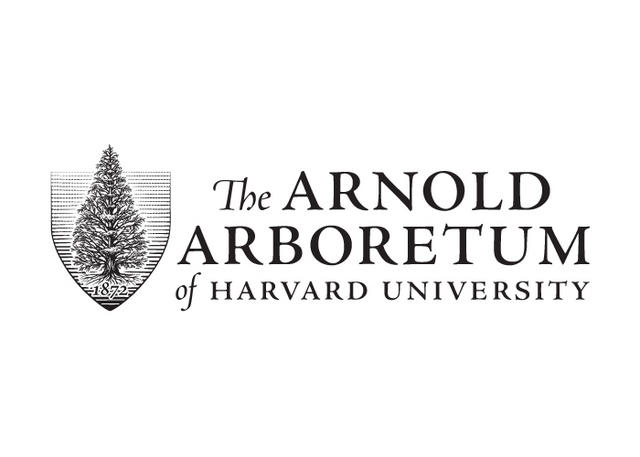
\includegraphics[width=0.2\textwidth]{/Users/danielbuonaiuto/Desktop/AA_logo.jpg}
\pagenumbering{gobble}
\\\\
\noindent{Dear Dr. Ellison,}\\
\vspace{1.5ex}

\noindent Please consider this manuscript ``Experimental designs for testing the interactive effects of temperature and light in ecology and the problem of periodicity" as a ``Perspective" article in \textit{Methods in Ecology and Evolution}.\\

\noindent Experiments in growth chambers or other controlled environments are a powerful tool for quantifying the individual and interactive effects of environmental cues on numerous biological processes. These studies have tremendously advanced our understanding of both fundamental eco-physiology and applied ecological forecasting \citep{Osmond:2004wb}. Yet, because experimentalists must balance ecological realism with statistical inference, experimental effort with statistical power, and account for the effects of unmanipulated or unmeasured variables \citep{schneiner2001}, seemingly small choices about experimental design can generate significant differences in outcomes. Using almost a century-worth experiments with the phenology of woody plants as a case study \citep{wolkovich2019}, our submission highlights how a commonly used experimental design aimed to partition the effects of temperature and photoperiod on spring phenology introduces experimental covariation into studies by coupling the periodicity of the light and temperature treatments, resulting in the incorrect estimation of cue effects. Notably, we examine the literature and find that up to 40\% of phenology studies have this issues, which may impart explain why the relative importance of photoperiod to spring phenology is a currently topic of significant controversy in the phenology literature \citep{koerner2010a,CHUINE:2010wg,Jennifer:2010un,Zohner:2016uz,WAY:2015aa}. \\

\noindent In this submission, we identify the extent of this problem by combining data simulations and an algebraic solution with a comparative analysis of published studies, but most importantly, we provide guidance for alternative experimental designs that can overcome this statistical issues. While we use spring phenology as a case study, we believe that our submission would be of broad interest to the readers of \textit{Methods in Ecology and Evoltion}, as it is relevant to any branch of ecology or evolutionary biology where light or temperature controls a biological response \citep[e.g.,][]{Franklin:2009wo,Brown:2014vn,Casal:2018us}.\\

\noindent Our submission provides both a concise overview of the basic requirements for testing interactions between environmental variables in experiments and a deep dive into an overlooked issue about how to include the periodicity of both light and temperature treatments in experiments. While there are many excellent books about designing ecological experiments, this duel focus makes this submission an important starting point for experimentalists, and has potentially to substantially improve our field's ability to accurate quantify the effects of temperature and light on a variety of ecological and evolutionary responses. \\

\noindent The main text of this manuscript is 2,942 words in length and it contains 4 figures. It is co-authored by M. Donohue and E.M. Wolkovich, and is not under consideration elsewhere. We hope that you will find it suitable for publication in \textit{Methods in Ecology and Evolution}, and look forward to hearing from you.\\\\ 
\\Sincerely,\\\\\\\\\\

\noindent Daniel Buonaiuto\\

\bibliography{..///refs/periodicity.bib}


\end{document}
